\documentclass{book}
\usepackage{amsmath, amsthm, amssymb}
\usepackage{graphicx}
\usepackage{hyperref}
\graphicspath{ {images/} }

\title{Data Mining on Massive Dataset}
\author{Nickson Zhu \\ \url{nicksonsone@gmail.com}}

\begin{document}
\maketitle
\tableofcontents
\newpage

\chapter{MapReduce}
Architecture:

Linux nodes = processor + main menory + disk.  Gigabit Ethernet 
interconnect.  Show as \ref{fig:cluster-archi}, a bunch of nodes is a rack.  
\begin{figure}[h]
	\centering
	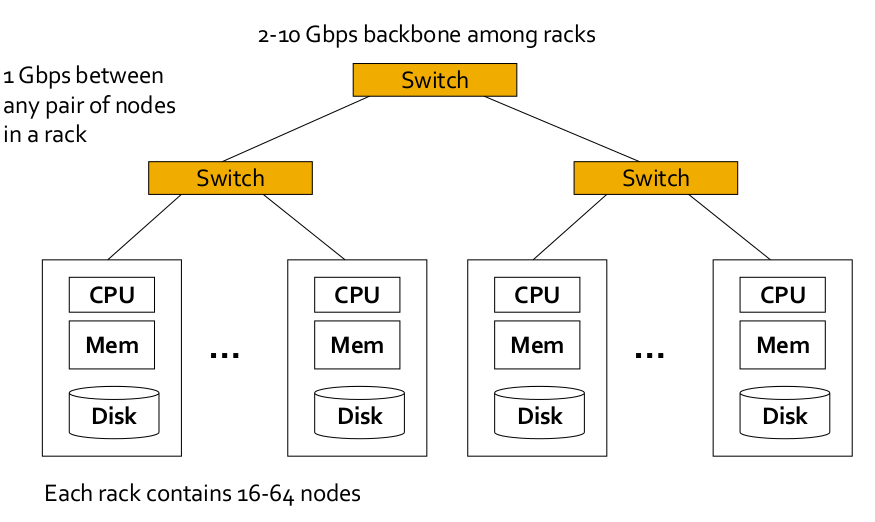
\includegraphics[scale=0.5]{cluster-archi}
	\label{fig:cluster-archi}
\end{figure}

Storing:

File is split into chuncks and each chunck is replicated.  Replicas are kept 
in different racks.  As shown in \ref{fig:store-files}
\begin{figure}[h]
	\centering
	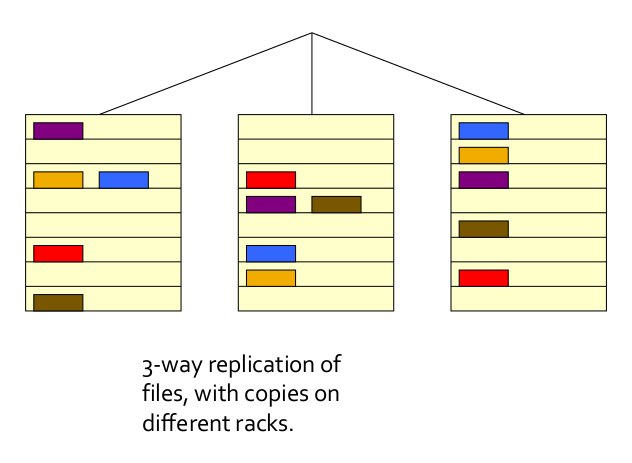
\includegraphics[scale=0.5]{store-files}
	\label{fig:store-files}
\end{figure}



\end{document}
